% AGH laboratory report. Engine: pdfLaTeX; bibliography: Biber.
% Content lives in content/, presentation in shared/style/universityreport.sty.
\documentclass[11pt,a4paper,oneside]{article}
\usepackage{universityreport}
\usepackage{hyperref}
\addbibresource{references.bib}
\graphicspath{{figures/}{generated/}{../../figures/}{../figures/}}
\usepackage{float}

% Required metadata. Keep plain text in title and author for PDF properties.
\reportinstitution{Akademia Górniczo-Hutnicza im. Stanisława Staszica w Krakowie}
\reportfaculty{Wydział Inżynierii Mechanicznej i Robotyki}
\reportprogramme{Inżynieria Akustyczna}
\reportcourse{Wibroakustyka w Technice i Środowisku 1}
\reporttitle{Hałas obiektu przemysłowego - pomiary w środowisku}
\reportlabnumber{1}
\reportauthor{Wojciech Salamak, Amelia Sowa}
\reportgroup{Grupa 2}
\reportinstructor{dr hab. inż. Janusz Piechowicz}
\reportdate{\today} % Date of exercise/submission: replace when needed.

% Optional metadata; empty values are hidden.
\reportlogo{agh_small.jpg}
\reporttype{Sprawozdanie laboratoryjne} % Or: Raport techniczny
\reportsubtitle{}
\reportsemester{}
\reportmeta{Wersja robocza -- z udokumentowanymi ograniczeniami pomiarów}

\begin{document}
\makecoverpage
% For longer technical reports, uncomment the optional elements:
% % Optional: enable in main.tex for a longer technical report.
\section*{Streszczenie}
\addcontentsline{toc}{section}{Streszczenie}
Krótko opisać cel, zastosowaną metodę, najważniejszy wynik
oraz wniosek końcowy. Uzupełnić po napisaniu raportu.

% \tableofcontents

\section{Cel i zakres ćwiczenia}
\label{sec:cel}
Celem ćwiczenia było wyznaczenie poziomu dźwięku A związanego
z pracą stacji gazowej nr 08/3159, zlokalizowanej przy skrzyżowaniu
ulic Oleandry i Romana Ingardena w Krakowie, w wybranym punkcie jej
otoczenia, z uwzględnieniem tła akustycznego.

Zastosowano metodę próbkowania opisaną w instrukcji laboratoryjnej
\autocite{piechowicz-konspekt}. Zakres opracowania obejmuje opis
obiektu i otoczenia, lokalizację stanowisk, charakterystykę aparatury,
opracowanie zapisanych próbek oraz ocenę ograniczeń przeprowadzonych
badań. Odstępstwa od wymagań instrukcji przedstawiono w dalszej
części sprawozdania.

\section{Charakterystyka obiektu i terenu}
\label{sec:obiekt}

\subsection{Opis badanego obiektu}
Badanym obiektem była stacja gazowa nr 08/3159. Pomiary wykonano
w jej otoczeniu, bez wyłączania instalacji. Nie przeprowadzono
inwentaryzacji urządzeń wewnątrz stacji, dlatego nie przypisano
zmierzonego hałasu konkretnym elementom jej wyposażenia.

\begin{figure}[H]
    \centering
    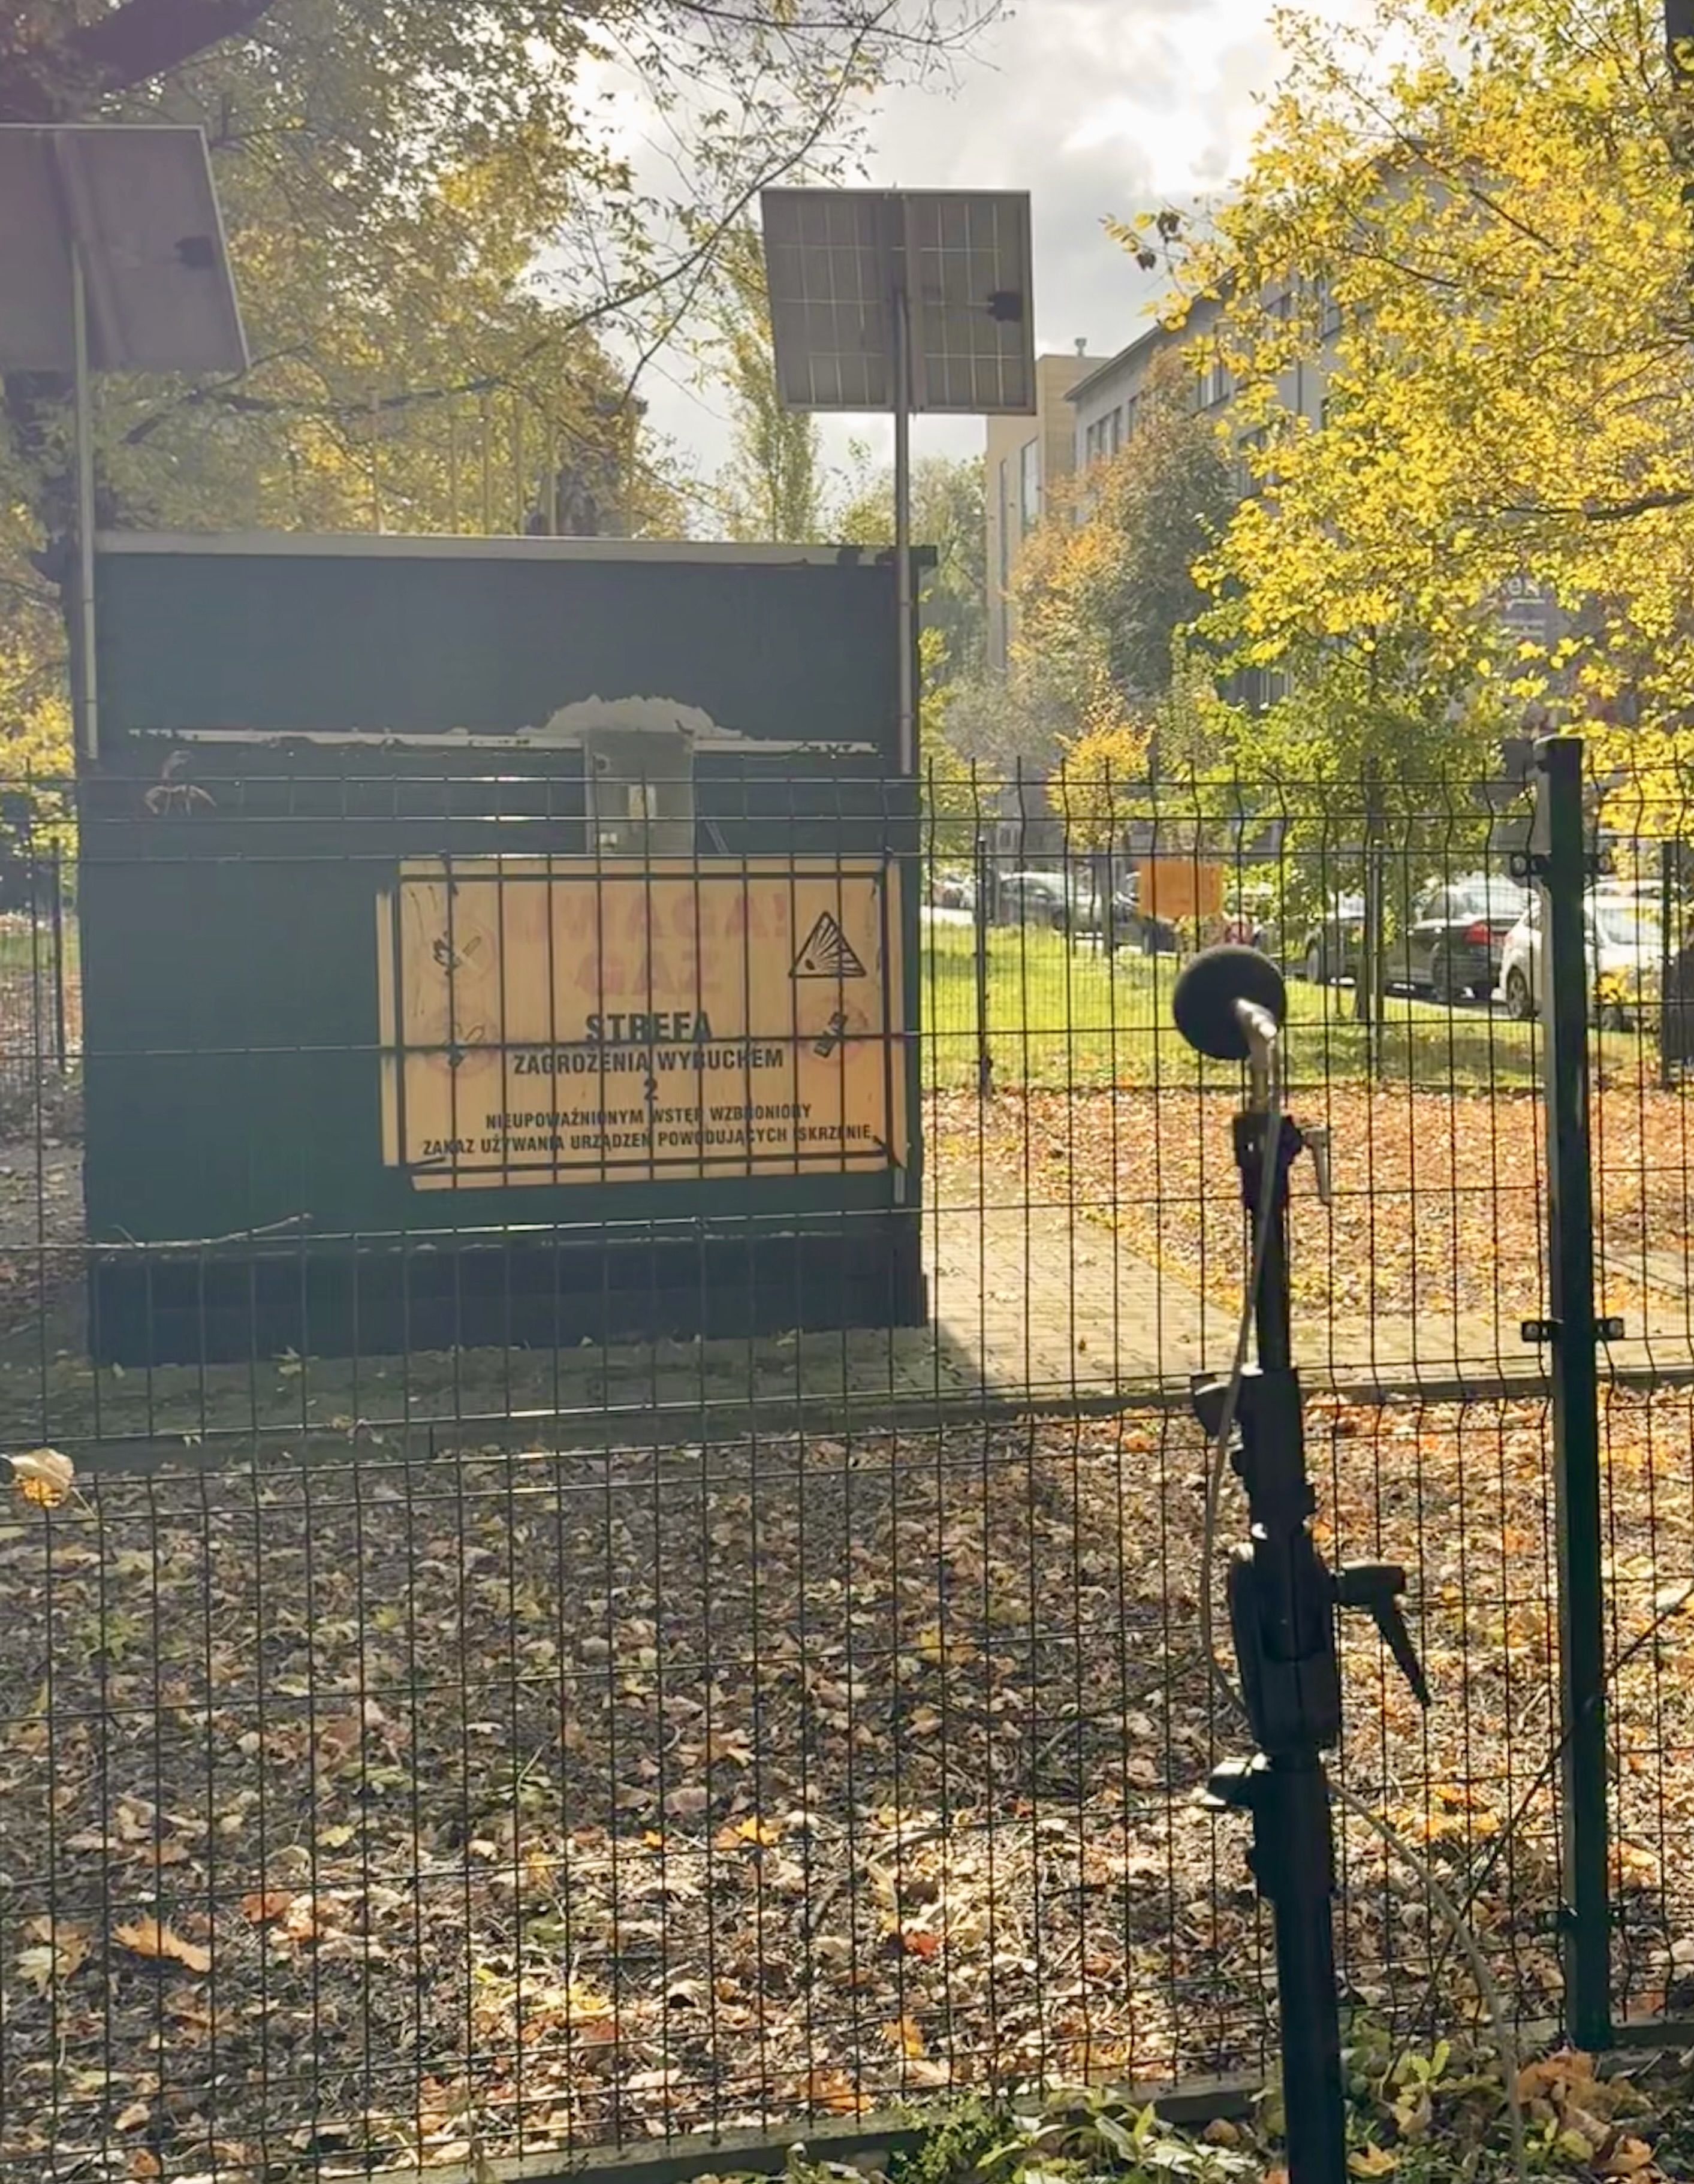
\includegraphics[width=0.5\linewidth,
        trim={0cm 10cm 5cm 30cm}, clip]{stacja_gazowa_mikrofon.jpeg}
    \caption{Stanowisko pomiarowe przy stacji gazowej nr 08/3159}
    \label{fig:stacja}
\end{figure}

\clearpage
\subsection{Charakterystyka otoczenia}
Według identyfikacji wykonanej podczas ćwiczenia stacja należy do
Polskiej Spółki Gazownictwa. Znajduje się na terenie zielonym,
w sąsiedztwie budynku Wydziału Inżynierii Środowiska i Geodezji
Uniwersytetu Rolniczego oraz ulic Oleandry i Romana Ingardena.
Ruch uliczny w pobliżu stacji stanowił potencjalne źródło zakłóceń w rejestrowanym sygnale. Nie dysponowano ilościowymi danymi o natężeniu ruchu.
Rozpatrywany w ćwiczeniu kierunek potencjalnej zabudowy nie stanowi
potwierdzenia przeznaczenia terenu w miejscowym planie
zagospodarowania przestrzennego.

\begin{figure} [H]
    \centering
    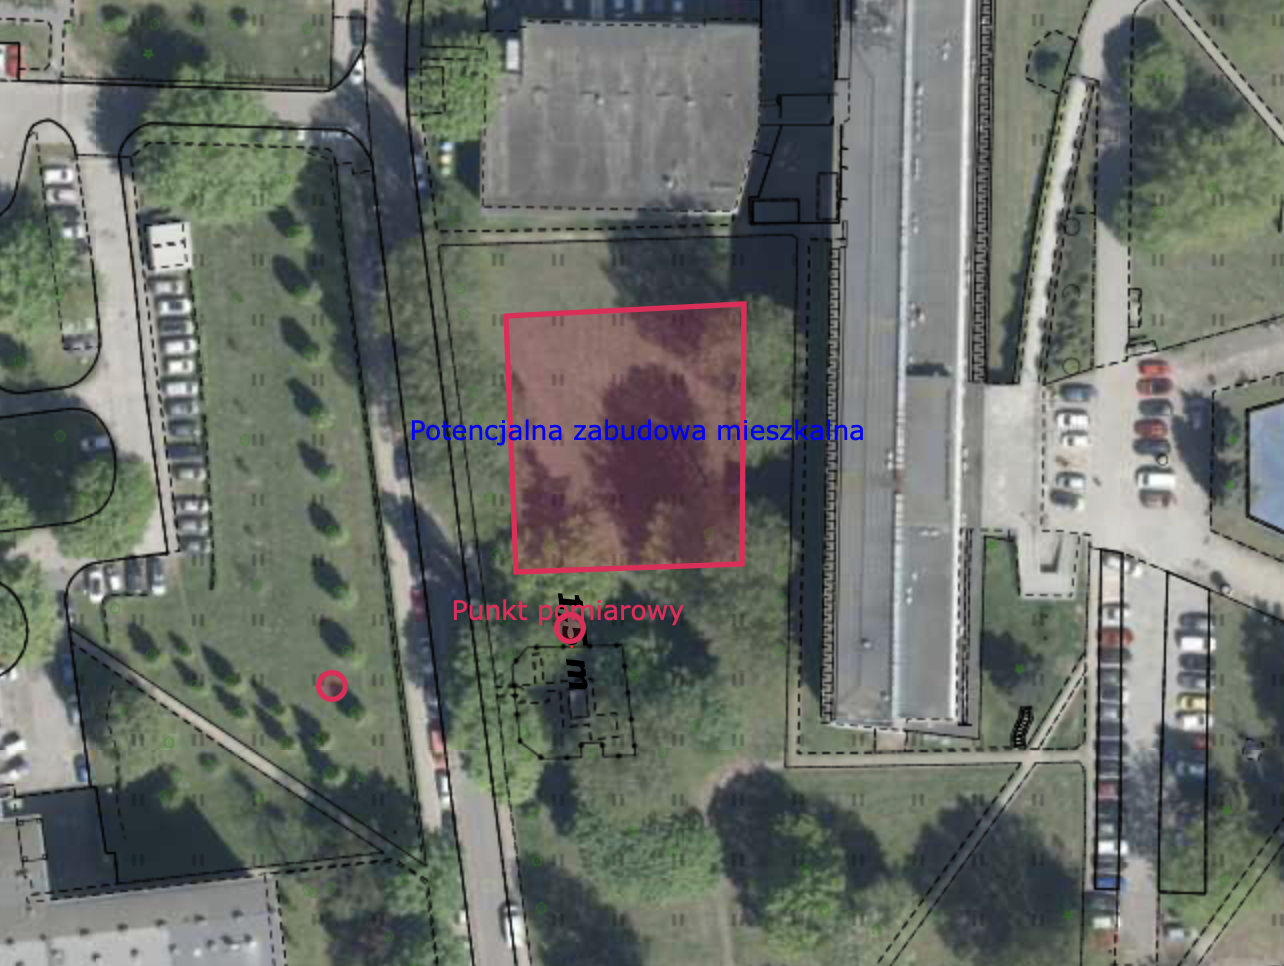
\includegraphics[width=0.5\linewidth]{potencjalna zabudowa.png}
    \caption{Usytuowanie stacji gazowej względem punktu pomiarowego i sąsiedniej zabudowy}
    \label{fig:otoczenie}
\end{figure}


\subsection{Lokalizacja punktów pomiarowych}
Punkt pomiaru hałasu zlokalizowano po północnej stronie stacji,
w odległości około $1{,}5\,\mathrm{m}$ od wskazanej podczas ćwiczenia
granicy obiektu. Mikrofon znajdował się na wysokości
$1{,}5\,\mathrm{m}$ nad gruntem. Punkt wybrano po stronie
rozpatrywanego kierunku potencjalnej zabudowy. Wynik charakteryzuje
to stanowisko; nie jest bezpośrednim pomiarem poziomu hałasu na
terenie odległej zabudowy.

\begin{figure}[H]
    \centering
    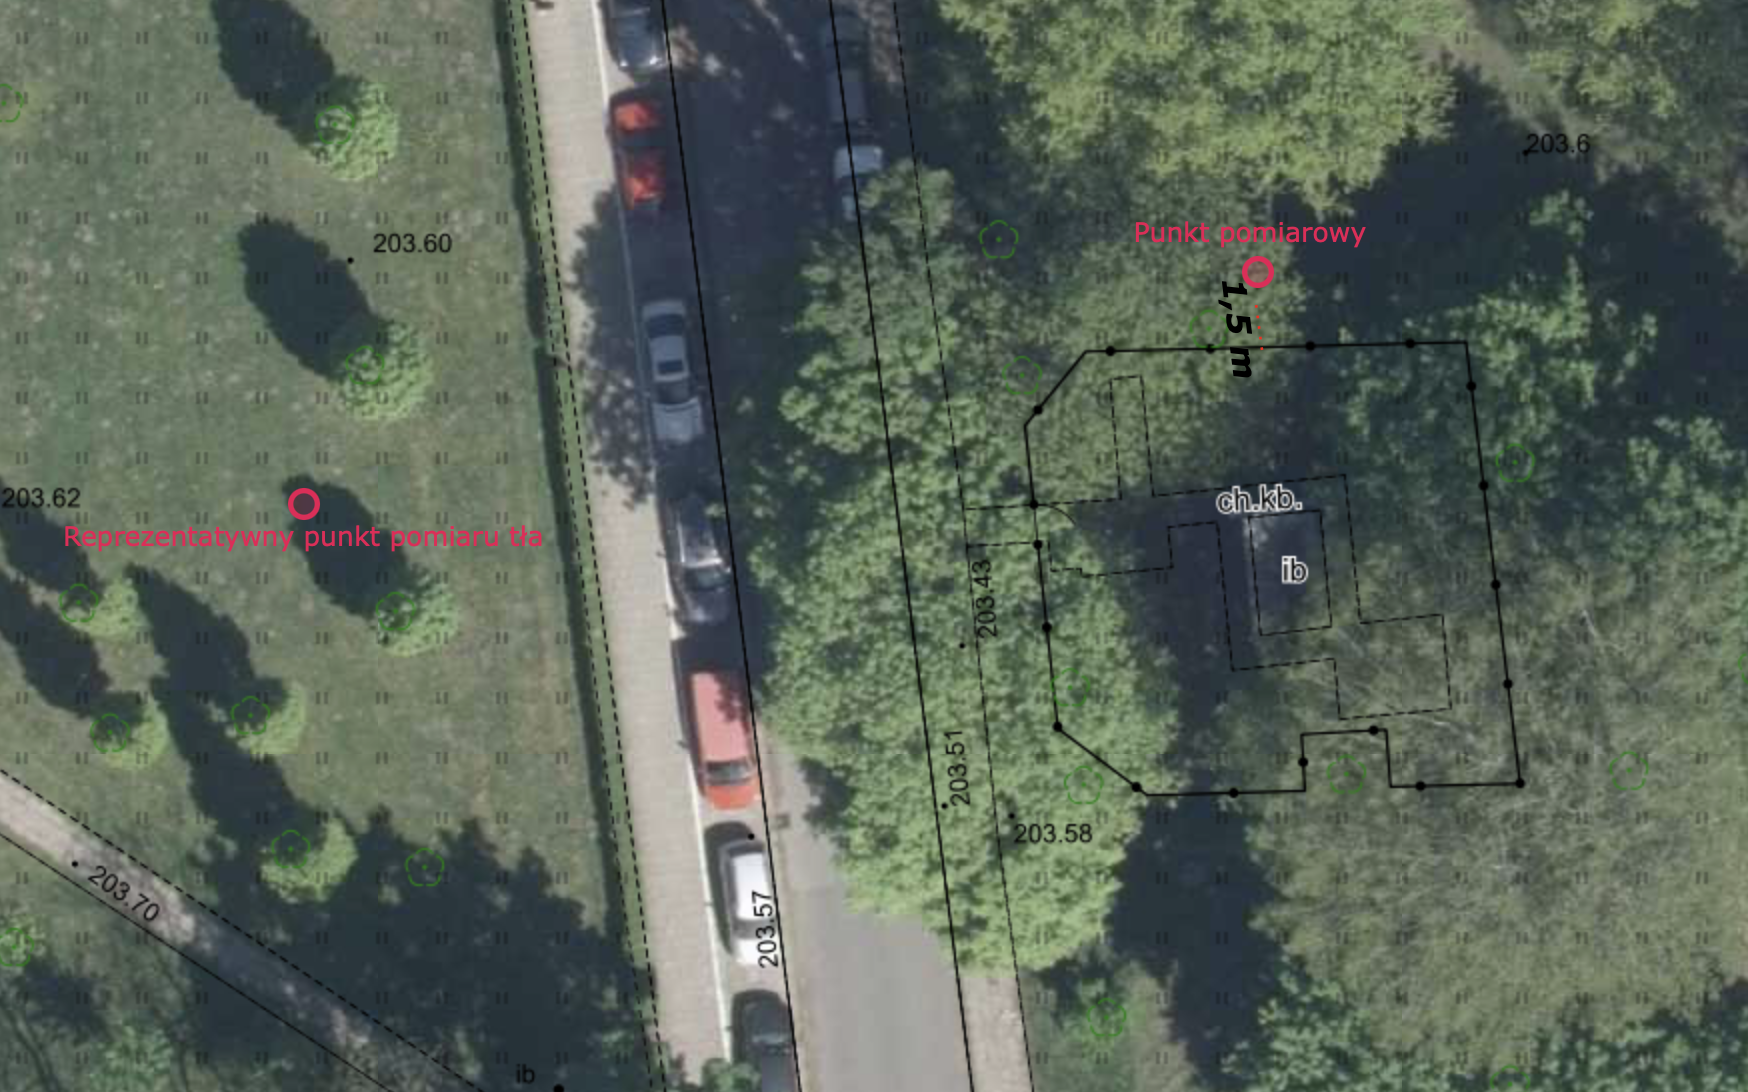
\includegraphics[width=0.8\linewidth]{punkty_pomiarowe.png}
    \caption{Lokalizacja punktu pomiaru hałasu oraz punktu pomiaru tła }
    \label{fig:punkty_pomiarowe}
\end{figure}

\subsection{Tło akustyczne}
Punkt pomiaru tła zaznaczono na rysunku~\ref{fig:punkty_pomiarowe}.
Ze względu na brak możliwości wstrzymania pracy stacji pomiar tła
wykonano w innym miejscu, po serii zasadniczej. Do pomiaru przy
stacji należą pliki P04--P08, a do pomiaru tła pliki P10--P14.
Nie udokumentowano ilościowo porównywalności oddziaływania źródeł
tła w obu punktach. Stanowi to ograniczenie interpretacji korekcji
tła akustycznego.

\section{Aparatura i warunki pomiaru}
\label{sec:aparatura}
\begin{table}[H]
 \centering
 \caption{Aparatura i wyposażenie wykorzystane podczas ćwiczenia.}
 \label{tab:aparatura}
 \begin{tabularx}{\linewidth}{@{}L L L@{}}
 \toprule
 Element & Oznaczenie & Informacja identyfikacyjna \\
 \midrule
 Miernik poziomu dźwięku & SVAN 971 & Nr seryjny 40452 \\
 Mikrofon pomiarowy & Pojemnościowy & --- \\
 Osłona przeciwwietrzna & --- & --- \\
 \bottomrule
 \end{tabularx}
\end{table}
Instrukcja producenta opisuje SVAN 971 jako miernik klasy 1
\autocite{svan971-manual}. Nie udostępniono danych świadectwa
wzorcowania używanego zestawu.

W obliczeniach wykorzystano pierwszy profil: korekcję
częstotliwościową A, detektor Fast i liniowe całkowanie poziomu
równoważnego. Czas integracji wynosił $10\,\mathrm{s}$,
a krok loggera $1\,\mathrm{s}$.

Przed sesją i po niej nie wykonano sprawdzenia toru kalibratorem,
ponieważ kalibrator nie został udostępniony przez prowadzącego.
Nie dysponowano wynikami sprawdzenia toru w dniu ćwiczenia.

\section{Metodyka}
\label{sec:metodyka}
\subsection{Przebieg pomiarów}
Po oględzinach obiektu i jego otoczenia wybrano stanowiska
pomiaru hałasu oraz tła. Zespoły laboratoryjne realizowały różne
warianty pomiaru; nasz zespół wykonywał próbki o czasie
$t_0=10\,\mathrm{s}$. Zarejestrowano pięć próbek przy stacji
oraz pięć próbek tła, z zastosowaniem osłony przeciwwietrznej.
Pracy stacji nie przerywano.
Dla każdej próbki przyjęto zarejestrowany przez miernik
równoważny poziom dźwięku A, $L_{Aeq,10s}$.

W instrukcji próbka $10\,\mathrm{s}$ jest przewidziana dla hałasu
stałego, gdy okresowe zakłócenia uniemożliwiają wykonanie próbki
$60\,\mathrm{s}$ między tymi zdarzeniami
\autocite{piechowicz-konspekt}.


\subsection{Obliczenia i kontrola liczby próbek}
Dla każdej serii wyznaczono rozstęp
\begin{equation}
 R=\max L_{Ak}-\min L_{Ak},
\end{equation}
gdzie $L_{Ak}$ oznacza wynik $k$-tej próbki o czasie $t_0$.
Liczbę próbek porównano z tabelą w instrukcji:
\begin{center}
\begin{tabular}{@{}lccccc@{}}
\toprule
$R$ [dB] & $(0;1]$ & $(1;1{,}5]$ & $(1{,}5;2]$ & $(2;2{,}5]$ & $(2{,}5;3]$ \\
Wymagane $n$ & 3 & 4 & 5 & 6 & 7 \\
\bottomrule
\end{tabular}
\end{center}
Przy $R>3\,\mathrm{dB}$ instrukcja przewiduje wydłużenie czasu
próbki.

Średnią dla próbek o jednakowym czasie trwania obliczono
energetycznie:
\begin{equation}
 L_{A\mathrm{sr}}=10\log_{10}\left(
 \frac{1}{n}\sum_{k=1}^{n}10^{0{,}1L_{Ak}}\right).
 \label{eq:srednia-energetyczna}
\end{equation}
Analogicznie wyznaczono średni poziom tła $L_{At}$.
Następnie obliczono różnicę $\Delta L=L_{A\mathrm{sr}}-L_{At}$
i zastosowano korekcję:
\begin{equation}
 L_{Aek}=10\log_{10}\left(
 10^{0{,}1L_{A\mathrm{sr}}}-10^{0{,}1L_{At}}\right).
 \label{eq:korekcja-tla}
\end{equation}
Instrukcja wymaga przy $\Delta L<3\,\mathrm{dB}$ zastosowania
metody obliczeniowej, a przy $\Delta L>10\,\mathrm{dB}$ dopuszcza
pominięcie tła.

\subsection{Warunki atmosferyczne}
\label{sec:warunki-atmosferyczne}
Podczas pomiarów panowały następujące warunki atmosferyczne:
\begin{itemize}
 \item temperatura otoczenia: $12{,}6\,^{\circ}\mathrm{C}$,
 \item ciśnienie atmosferyczne: $999{,}5\,\mathrm{hPa}$,
 \item prędkość wiatru: $2\,\mathrm{m/s}$,
 \item wilgotność względna: $55{,}11\,\%$.
\end{itemize}
Dane o warunkach atmosferycznych pozyskane ze strony \href{https://meteo.fis.agh.edu.pl.}{ Meteo Fis AGH}.
\section{Wyniki pomiarów}
\label{sec:wyniki}
W tabeli~\ref{tab:wyniki} zestawiono wszystkie dostępne próbki
zarejestrowane miernikiem. Każda próbka trwała $10\,\mathrm{s}$.
Wartości odnoszą się do profilu A i liniowego całkowania Leq.
\begin{table}[htbp]
 \centering
 \caption{Równoważne poziomy dźwięku A w próbkach $10\,\mathrm{s}$.}
 \label{tab:wyniki}
 \begin{tabular}{@{}lrlr@{}}
\toprule
Plik: stacja & $L_{Aeq,10s}$ [dB] & Plik: tło & $L_{Aeq,10s}$ [dB] \\
\midrule
P04 & 52,54 & P10 & 48,05 \\
P05 & 52,27 & P11 & 47,72 \\
P06 & 51,96 & P12 & 49,77 \\
P07 & 53,31 & P13 & 47,08 \\
P08 & 53,42 & P14 & 47,20 \\
\bottomrule
\end{tabular}

\end{table}


\begin{table}[htbp]
 \centering
 \caption{Opracowanie serii i sprawdzenie wymaganej liczby próbek.}
 \label{tab:opracowanie}
 \begin{tabular}{@{}lrr@{}}
\toprule
Wielkość & Przy stacji \\
\midrule
Średnia energetyczna [dB] & 52,74 \\
Rozstęp $R$ [dB] & 1,46  \\
Liczba wykonanych próbek & 5  \\
Wymagana liczba próbek & 4  \\
Kryterium liczby próbek & spełnione  \\
\bottomrule
\end{tabular}

\end{table}
Seria zasadnicza spełnia kryterium liczby próbek. 

Różnica średnich poziomów wyniosła $\Delta L=4,66\,\mathrm{dB}$.
Po podstawieniu do wzoru~\eqref{eq:korekcja-tla} otrzymano
\begin{equation}
 L_{Aek}=50,92\,\mathrm{dB}.
\end{equation}

Ze względu na brak sprawdzenia toru
kalibratorem oraz brak pełnej dokumentacji warunków wynik ten
należy traktować jako oszacowanie dla warunków ćwiczenia.
Nie stanowi on podstawy do stwierdzenia dotrzymania lub przekroczenia
poziomu dopuszczalnego na terenie chronionym przed hałasem.

% Rozdział o niepewności pominięto: brak danych o zestawie pomiarowym.
\clearpage
\section{Wnioski}
\label{sec:wnioski}
\begin{enumerate}
 \item Dla pięciu próbek przy stacji gazowej uzyskano średni
 energetyczny poziom $52{,}74\,\mathrm{dB}$, a dla pięciu próbek
 tła $48{,}08\,\mathrm{dB}$. Różnica wyniosła $4{,}66\,\mathrm{dB}$,
 dlatego wpływ tła wymagał uwzględnienia.
 \item Po korekcji tła otrzymano robocze oszacowanie poziomu
 związanego z pracą stacji $L_{Aek}\approx50{,}9\,\mathrm{dB}$.
 Wynik charakteryzuje wybrany punkt i warunki krótkiej serii
 pomiarowej.
 \item Seria przy stacji spełnia kryterium liczby próbek z instrukcji.
 Dla serii tła wymagane było siedem próbek, a dostępnych jest pięć.
 Jest to niezrealizowany element procedury.
 \item Nie przeprowadzono sprawdzenia toru kalibratorem przed
 sesją ani po niej, ponieważ nie był on dostępny. Brak dokumentacji
 wzorcowania i danych meteorologicznych ogranicza ocenę
 wiarygodności wyników.
\end{enumerate}

\printbibliography[heading=bibintoc,title={Literatura}]

% Optional supplementary material:
% \appendix
% % Optional: enable after \\appendix in main.tex.
\section{Materiały uzupełniające}
\label{sec:zalacznik}
Zamieścić dodatkowe dane, obliczenia lub kod niezbędny do odtworzenia analizy.
\begin{lstlisting}[language=Python,caption={Przykład obliczenia średniej i niepewności typu A.},label={lst:analiza}]
import csv
from statistics import mean, stdev
from math import sqrt

with open("data/raw/measurements.csv", encoding="utf-8") as stream:
    levels = [float(row["level"]) for row in csv.DictReader(stream)]
print(mean(levels), stdev(levels) / sqrt(len(levels)))
\end{lstlisting}

\end{document}
